\chapter[Gomory cuts]{}
\section{Famiglie di tagli}

Branch-and-bound → Branch-and-bound-and-cut   (prima si cerca di tagliare un po’ poi di fare branch)
\nt{
Rilassamento continuo di un problema ILP:

$$
\begin{array}{c}
    Z(L P)=\operatorname{Max} c^{\top} x \\
    A x = b \\
    x \geqslant 0\\
\end{array}
$$
}

\nt{
    \textbf{Dizionario ottimo:}

\[
\begin{cases}x_B+\tilde{A} x_{\bar{B}}=\tilde{b} & \tilde{A}=A_B^{-1} A_{\bar{B}} \\ \underbrace{c^{\top}}_{z} x=\psi+\underbrace{\tilde{C}_B^{\top}}_{\tilde{C}_B^T \leq 0} x_{\bar{B}} & \end{cases}
\]

\[
\tilde{A}=\left[\begin{array}{cccc}\tilde{a}_{11} & \tilde{a}_{12} & \ldots & \tilde{a}_{1(n-m)} \\\vdots & \cdots & & \\\tilde{a}_{n 1} & \tilde{a}_{n 2} & \ldots & a_m(n-m)\end{array}\right]\\ \text{m righe}\\ \text{n-m colonne}
\]
}

\section{Gomory cuts}

\[
\begin{aligned}\tilde{A}_i & =\left[\tilde{a}_{i 2}, \ldots ,\tilde{a}_i(n-m)\right] \\{\lfloor\tilde{A}_i\rfloor } & =\left[\lfloor a_{i 2}\rfloor, \ldots,\left \lfloor\tilde{a}_i(n-m)\rfloor\right]\right.\end{aligned}
\]

Prendiamo la riga i-esima del dizionario ottimo: $\forall i \in\{1, \ldots, m\}$
\[
\begin{array}{c}
    (II) x_B^i+\tilde{A}_i x_{\bar{B}}=\tilde{b}_i \\ \\ \text{Dato che le variabili sono tutte negative abbiamo:}\\\left\lfloor \tilde{A}_i\right\rfloor x_{\bar{B}} \leqslant \tilde{A}_i x_{\bar{B}} \ \text{Allora}\ x_B^i+\left\lfloor\tilde{A}_i\right\rfloor x_{\bar{B}} \leqslant \tilde{b}_i \\  \\ \text{Dato che le variabili devono essere intere:}\\x_B^i+\lfloor\tilde{A}_i \rfloor x_{\bar{b}} \leqslant\lfloor\tilde{b}_i\rfloor \quad (I) \\ \text{Sottraendo II e I}\\ (\tilde{A}_i-\lfloor\tilde{A}_i\rfloor) x_{\bar{B}} \geqslant \tilde{b}_i-\lfloor\tilde{b}_i\rfloor \ \ (\geq\text{ perchè togliamo più a dx che sx})\\ \text{Taglio di Gomery alla riga i}
\end{array}
\]

I tagli di Gomory assicurano che la soluzione in base ammissibile $x_B=\tilde{B}\geqslant0$ 
diventa infeasible → ma non tagliano nessuna soluzione intera

\textbf{Cutting plan}→ Soluzione intera trovata con solo tagli

\nt{
    Parte intera di un numero reale:

    $y \in \mathbb{R}, \lfloor y\rfloor=\text{Max intero } q*q \leqslant y$
}

\ex{Esempi di tagli}{
\[
\begin{array}{c}
\underbrace{\left(-\frac{1}{5}-\left(\frac{1}{5}\right)\right)}_{\frac{4}{5}}x_3   +\underbrace{\left(\frac{1}{10}-\left\lfloor\frac{1}{10}\right\rfloor\right)}_{\frac{1}{10}}x_4\geqslant \underbrace{\left(\frac{3}{2}-\left\lfloor\frac{3}{2}\right\rfloor\right)}_{\frac{1}{2}}\rightarrow 8 x_3+x_4 \geq 5
\\(\underbrace{\left(\frac{4}{5}-\left(\frac{1}{5}\right)\right.}_{\frac{4}{5}}) x_3+\underbrace{\left(\frac{1}{10}+\left(\frac{1}{10}\right)\right.}_{\frac{1}{10}}) x_4)(\underbrace{\left.\frac{7}{2}-\left(\frac{7}{2}\right)\right)}_{\frac{1}{2}} \rightarrow 8 x_3+x_4 \geq 5
\end{array}
\]

\[
\begin{aligned}& x_3=2+x_1-x_2 \quad x_4=19-8 x_1-2 x_2 \\& 8\left(2+x_1-x_2\right)+\left(19-8 x_1-2 n_2\right) \geqslant 5 \rightarrow \fcolorbox{red}{white}{$x_2 \leq 3$}\end{aligned}
\]

\[
\begin{aligned}& \tilde{x}_1=\frac{13}{8}, \tilde{x}_2=3 \\& z(L P)=\frac{37}{8} \geqslant z(L P)\end{aligned}
\]
\begin{center}
    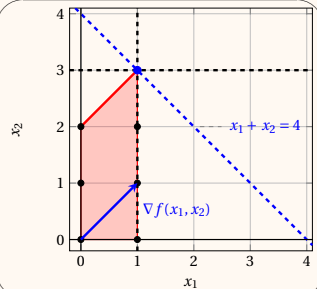
\includegraphics[height=3cm]{gc1}
    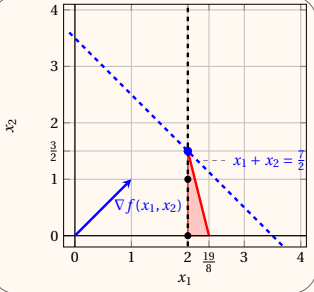
\includegraphics[height=3cm]{gc2}
\[
\begin{aligned}& \tilde{x}_1=\frac{13}{8}, \tilde{x}_2=3 \\& z(L P)=\frac{37}{8} \geqslant z(L P)\end{aligned}
\]
\end{center}

\begin{center}
    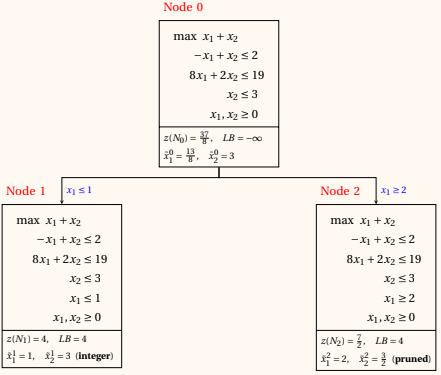
\includegraphics[height=8cm]{alb}
\end{center}
}

